\documentclass[]{article}
\usepackage{lmodern}
\usepackage{amssymb,amsmath}
\usepackage{ifxetex,ifluatex}
\usepackage{fixltx2e} % provides \textsubscript
\ifnum 0\ifxetex 1\fi\ifluatex 1\fi=0 % if pdftex
  \usepackage[T1]{fontenc}
  \usepackage[utf8]{inputenc}
\else % if luatex or xelatex
  \ifxetex
    \usepackage{mathspec}
  \else
    \usepackage{fontspec}
  \fi
  \defaultfontfeatures{Ligatures=TeX,Scale=MatchLowercase}
\fi
% use upquote if available, for straight quotes in verbatim environments
\IfFileExists{upquote.sty}{\usepackage{upquote}}{}
% use microtype if available
\IfFileExists{microtype.sty}{%
\usepackage{microtype}
\UseMicrotypeSet[protrusion]{basicmath} % disable protrusion for tt fonts
}{}
\usepackage[margin=1in]{geometry}
\usepackage{hyperref}
\hypersetup{unicode=true,
            pdftitle={01\_normalisation},
            pdfauthor={Aurelien Dugourd},
            pdfborder={0 0 0},
            breaklinks=true}
\urlstyle{same}  % don't use monospace font for urls
\usepackage{color}
\usepackage{fancyvrb}
\newcommand{\VerbBar}{|}
\newcommand{\VERB}{\Verb[commandchars=\\\{\}]}
\DefineVerbatimEnvironment{Highlighting}{Verbatim}{commandchars=\\\{\}}
% Add ',fontsize=\small' for more characters per line
\usepackage{framed}
\definecolor{shadecolor}{RGB}{248,248,248}
\newenvironment{Shaded}{\begin{snugshade}}{\end{snugshade}}
\newcommand{\AlertTok}[1]{\textcolor[rgb]{0.94,0.16,0.16}{#1}}
\newcommand{\AnnotationTok}[1]{\textcolor[rgb]{0.56,0.35,0.01}{\textbf{\textit{#1}}}}
\newcommand{\AttributeTok}[1]{\textcolor[rgb]{0.77,0.63,0.00}{#1}}
\newcommand{\BaseNTok}[1]{\textcolor[rgb]{0.00,0.00,0.81}{#1}}
\newcommand{\BuiltInTok}[1]{#1}
\newcommand{\CharTok}[1]{\textcolor[rgb]{0.31,0.60,0.02}{#1}}
\newcommand{\CommentTok}[1]{\textcolor[rgb]{0.56,0.35,0.01}{\textit{#1}}}
\newcommand{\CommentVarTok}[1]{\textcolor[rgb]{0.56,0.35,0.01}{\textbf{\textit{#1}}}}
\newcommand{\ConstantTok}[1]{\textcolor[rgb]{0.00,0.00,0.00}{#1}}
\newcommand{\ControlFlowTok}[1]{\textcolor[rgb]{0.13,0.29,0.53}{\textbf{#1}}}
\newcommand{\DataTypeTok}[1]{\textcolor[rgb]{0.13,0.29,0.53}{#1}}
\newcommand{\DecValTok}[1]{\textcolor[rgb]{0.00,0.00,0.81}{#1}}
\newcommand{\DocumentationTok}[1]{\textcolor[rgb]{0.56,0.35,0.01}{\textbf{\textit{#1}}}}
\newcommand{\ErrorTok}[1]{\textcolor[rgb]{0.64,0.00,0.00}{\textbf{#1}}}
\newcommand{\ExtensionTok}[1]{#1}
\newcommand{\FloatTok}[1]{\textcolor[rgb]{0.00,0.00,0.81}{#1}}
\newcommand{\FunctionTok}[1]{\textcolor[rgb]{0.00,0.00,0.00}{#1}}
\newcommand{\ImportTok}[1]{#1}
\newcommand{\InformationTok}[1]{\textcolor[rgb]{0.56,0.35,0.01}{\textbf{\textit{#1}}}}
\newcommand{\KeywordTok}[1]{\textcolor[rgb]{0.13,0.29,0.53}{\textbf{#1}}}
\newcommand{\NormalTok}[1]{#1}
\newcommand{\OperatorTok}[1]{\textcolor[rgb]{0.81,0.36,0.00}{\textbf{#1}}}
\newcommand{\OtherTok}[1]{\textcolor[rgb]{0.56,0.35,0.01}{#1}}
\newcommand{\PreprocessorTok}[1]{\textcolor[rgb]{0.56,0.35,0.01}{\textit{#1}}}
\newcommand{\RegionMarkerTok}[1]{#1}
\newcommand{\SpecialCharTok}[1]{\textcolor[rgb]{0.00,0.00,0.00}{#1}}
\newcommand{\SpecialStringTok}[1]{\textcolor[rgb]{0.31,0.60,0.02}{#1}}
\newcommand{\StringTok}[1]{\textcolor[rgb]{0.31,0.60,0.02}{#1}}
\newcommand{\VariableTok}[1]{\textcolor[rgb]{0.00,0.00,0.00}{#1}}
\newcommand{\VerbatimStringTok}[1]{\textcolor[rgb]{0.31,0.60,0.02}{#1}}
\newcommand{\WarningTok}[1]{\textcolor[rgb]{0.56,0.35,0.01}{\textbf{\textit{#1}}}}
\usepackage{graphicx,grffile}
\makeatletter
\def\maxwidth{\ifdim\Gin@nat@width>\linewidth\linewidth\else\Gin@nat@width\fi}
\def\maxheight{\ifdim\Gin@nat@height>\textheight\textheight\else\Gin@nat@height\fi}
\makeatother
% Scale images if necessary, so that they will not overflow the page
% margins by default, and it is still possible to overwrite the defaults
% using explicit options in \includegraphics[width, height, ...]{}
\setkeys{Gin}{width=\maxwidth,height=\maxheight,keepaspectratio}
\IfFileExists{parskip.sty}{%
\usepackage{parskip}
}{% else
\setlength{\parindent}{0pt}
\setlength{\parskip}{6pt plus 2pt minus 1pt}
}
\setlength{\emergencystretch}{3em}  % prevent overfull lines
\providecommand{\tightlist}{%
  \setlength{\itemsep}{0pt}\setlength{\parskip}{0pt}}
\setcounter{secnumdepth}{0}
% Redefines (sub)paragraphs to behave more like sections
\ifx\paragraph\undefined\else
\let\oldparagraph\paragraph
\renewcommand{\paragraph}[1]{\oldparagraph{#1}\mbox{}}
\fi
\ifx\subparagraph\undefined\else
\let\oldsubparagraph\subparagraph
\renewcommand{\subparagraph}[1]{\oldsubparagraph{#1}\mbox{}}
\fi

%%% Use protect on footnotes to avoid problems with footnotes in titles
\let\rmarkdownfootnote\footnote%
\def\footnote{\protect\rmarkdownfootnote}

%%% Change title format to be more compact
\usepackage{titling}

% Create subtitle command for use in maketitle
\providecommand{\subtitle}[1]{
  \posttitle{
    \begin{center}\large#1\end{center}
    }
}

\setlength{\droptitle}{-2em}

  \title{01\_normalisation}
    \pretitle{\vspace{\droptitle}\centering\huge}
  \posttitle{\par}
    \author{Aurelien Dugourd}
    \preauthor{\centering\large\emph}
  \postauthor{\par}
      \predate{\centering\large\emph}
  \postdate{\par}
    \date{5/11/2020}


\begin{document}
\maketitle

\hypertarget{license-info}{%
\subsubsection{License Info}\label{license-info}}

This program is free software: you can redistribute it and/or modify it
under the terms of the GNU General Public License as published by the
Free Software Foundation, either version 3 of the License, or (at your
option) any later version.

This program is distributed in the hope that it will be useful, but
WITHOUT ANY WARRANTY; without even the implied warranty of
MERCHANTABILITY or FITNESS FOR A PARTICULAR PURPOSE. See the GNU General
Public License for more details.

Please check \url{http://www.gnu.org/licenses/}.

\hypertarget{introduction}{%
\subsection{Introduction}\label{introduction}}

Here we present examples of normalisation strategies of omic dataset,
using RNAseq for the present case.

\hypertarget{getting-started}{%
\subsection{Getting Started}\label{getting-started}}

We first load the required libraries.

\begin{Shaded}
\begin{Highlighting}[]
\CommentTok{#Main libraries}
\KeywordTok{library}\NormalTok{(readr)}
\KeywordTok{library}\NormalTok{(vsn)}

\CommentTok{#Support functions also requires}
\KeywordTok{library}\NormalTok{(ggplot2)}
\KeywordTok{library}\NormalTok{(reshape)}
\KeywordTok{library}\NormalTok{(pheatmap)}
\KeywordTok{library}\NormalTok{(gridExtra)}
\KeywordTok{library}\NormalTok{(grid)}
\KeywordTok{library}\NormalTok{(cowplot)}
\KeywordTok{library}\NormalTok{(ggrepel)}
\KeywordTok{library}\NormalTok{(hexbin)}

\CommentTok{#Import the support funciton script }
\CommentTok{#/!\textbackslash{}/!\textbackslash{} PATH NEEDS TO BE ADAPTED /!\textbackslash{}/!\textbackslash{}}

\KeywordTok{source}\NormalTok{(}\StringTok{"scripts/support_functions.R"}\NormalTok{)}
\end{Highlighting}
\end{Shaded}

\hypertarget{import-the-raw-count-dataframe}{%
\subsubsection{Import the raw count
dataframe}\label{import-the-raw-count-dataframe}}

downloaded from
\url{https://www.ncbi.nlm.nih.gov/geo/query/acc.cgi?acc=GSE119931}
download the file : GSE119931\_PANC1.FOXA2KO.genes.counts.txt.gz and
decompress it in the data folder

\begin{Shaded}
\begin{Highlighting}[]
\NormalTok{## Raw counts table}
\NormalTok{GSE119931_PANC1_FOXA2KO_genes_counts <-}\StringTok{ }\KeywordTok{as.data.frame}\NormalTok{(}
  \KeywordTok{read_delim}\NormalTok{(}\StringTok{"data/GSE119931_PANC1.FOXA2KO.genes.counts.txt"}\NormalTok{, }
                                                   \StringTok{"}\CharTok{\textbackslash{}t}\StringTok{"}\NormalTok{, }\DataTypeTok{escape_double =} \OtherTok{FALSE}\NormalTok{, }\DataTypeTok{trim_ws =} \OtherTok{TRUE}\NormalTok{)) }
\end{Highlighting}
\end{Shaded}

\begin{verbatim}
## Parsed with column specification:
## cols(
##   Geneid = col_character(),
##   Chr = col_character(),
##   Start = col_character(),
##   End = col_character(),
##   Strand = col_character(),
##   Length = col_double(),
##   PANC1.WT.Rep1 = col_double(),
##   PANC1.WT.Rep2 = col_double(),
##   PANC1.WT.Rep3 = col_double(),
##   PANC1.FOXA2KO.Rep1 = col_double(),
##   PANC1.FOXA2KO.Rep2 = col_double(),
##   PANC1.FOXA2KO.Rep3 = col_double()
## )
\end{verbatim}

\begin{Shaded}
\begin{Highlighting}[]
\NormalTok{count_df <-}\StringTok{ }\NormalTok{GSE119931_PANC1_FOXA2KO_genes_counts[,}\KeywordTok{c}\NormalTok{(}\DecValTok{7}\OperatorTok{:}\DecValTok{12}\NormalTok{)]}
\KeywordTok{row.names}\NormalTok{(count_df) <-}\StringTok{ }\NormalTok{GSE119931_PANC1_FOXA2KO_genes_counts}\OperatorTok{$}\NormalTok{Geneid}
\end{Highlighting}
\end{Shaded}

\hypertarget{pre-processing-and-normalisation}{%
\subsubsection{Pre-processing and
normalisation}\label{pre-processing-and-normalisation}}

First create a dataframe to summarise experimental design called targets

\begin{Shaded}
\begin{Highlighting}[]
\NormalTok{targets <-}\StringTok{ }\KeywordTok{as.data.frame}\NormalTok{(}\KeywordTok{matrix}\NormalTok{(}\OtherTok{NA}\NormalTok{,}\KeywordTok{length}\NormalTok{(}\KeywordTok{names}\NormalTok{(count_df)),}\DecValTok{2}\NormalTok{))}
\KeywordTok{names}\NormalTok{(targets) <-}\StringTok{ }\KeywordTok{c}\NormalTok{(}\StringTok{"sample"}\NormalTok{,}\StringTok{"condition"}\NormalTok{)}
\NormalTok{targets}\OperatorTok{$}\NormalTok{sample <-}\StringTok{ }\KeywordTok{names}\NormalTok{(count_df)}
\NormalTok{targets}\OperatorTok{$}\NormalTok{condition <-}\StringTok{ }\KeywordTok{gsub}\NormalTok{(}\StringTok{".Rep[0-9]$"}\NormalTok{,}\StringTok{""}\NormalTok{,targets}\OperatorTok{$}\NormalTok{sample)}
\end{Highlighting}
\end{Shaded}

Make some plots to check what the data looks like after only a log2
transformation

\begin{Shaded}
\begin{Highlighting}[]
\CommentTok{#First we remove rows that contain only 0}
\NormalTok{count_df <-}\StringTok{ }\NormalTok{count_df[}\KeywordTok{rowSums}\NormalTok{(count_df) }\OperatorTok{>}\StringTok{ }\DecValTok{0}\NormalTok{,]}
\CommentTok{#remaining 0 have to be made as NA so that log2 transformation is possible}
\NormalTok{count_df[count_df }\OperatorTok{==}\StringTok{ }\DecValTok{0}\NormalTok{] <-}\StringTok{ }\OtherTok{NA}
\end{Highlighting}
\end{Shaded}

\begin{Shaded}
\begin{Highlighting}[]
\CommentTok{#make the plots}
\NormalTok{plots <-}\StringTok{ }\KeywordTok{magicPlotMakerLight}\NormalTok{(}\DataTypeTok{df =} \KeywordTok{log2}\NormalTok{(count_df), }\DataTypeTok{targets =}\NormalTok{ targets)}
\end{Highlighting}
\end{Shaded}

\begin{verbatim}
## Using ID as id variables
\end{verbatim}

\begin{verbatim}
## Warning: Using alpha for a discrete variable is not advised.

## Warning: Using alpha for a discrete variable is not advised.

## Warning: Using alpha for a discrete variable is not advised.

## Warning: Using alpha for a discrete variable is not advised.
\end{verbatim}

\begin{Shaded}
\begin{Highlighting}[]
\KeywordTok{plot}\NormalTok{(plots[[}\DecValTok{1}\NormalTok{]]) }\CommentTok{#violins}
\end{Highlighting}
\end{Shaded}

\begin{verbatim}
## Warning: Removed 18617 rows containing non-finite values (stat_ydensity).
\end{verbatim}

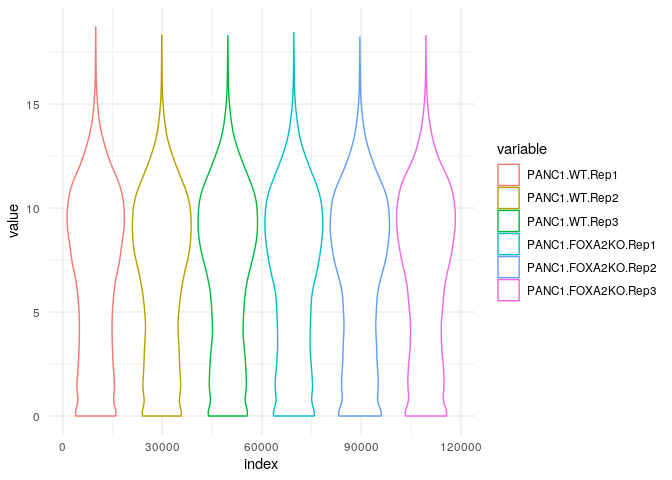
\includegraphics{01_normalisation_files/figure-latex/unnamed-chunk-5-1.pdf}

\begin{Shaded}
\begin{Highlighting}[]
\KeywordTok{plot}\NormalTok{(plots[[}\DecValTok{2}\NormalTok{]]) }\CommentTok{#PCA}
\end{Highlighting}
\end{Shaded}

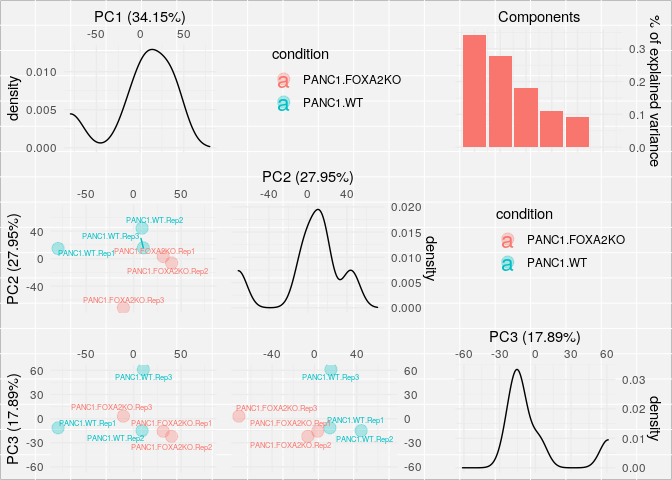
\includegraphics{01_normalisation_files/figure-latex/unnamed-chunk-5-2.pdf}

From the violin plot, we can see that the distributions are bimodal.
Usually this is because a lots of genes are expressed under the RNAseq
detection threshold and will give rise to a noisy sub-distribution. We
want to get rid of those reads, so based on the violin plot, we decide
to exclude any transcript with less that 4 log2(counts)

\begin{Shaded}
\begin{Highlighting}[]
\NormalTok{count_df[}\KeywordTok{log2}\NormalTok{(count_df) }\OperatorTok{<}\StringTok{ }\DecValTok{4}\NormalTok{ ] <-}\StringTok{ }\OtherTok{NA}

\CommentTok{#remove rows that don't have enough well measured genes in enough samples}
\NormalTok{count_df <-}\StringTok{ }\NormalTok{count_df[}\KeywordTok{rowSums}\NormalTok{(}\KeywordTok{is.na}\NormalTok{(count_df[,}\KeywordTok{c}\NormalTok{(}\DecValTok{1}\OperatorTok{:}\DecValTok{3}\NormalTok{)])) }\OperatorTok{<}\StringTok{ }\DecValTok{2}\NormalTok{,]}
\NormalTok{count_df <-}\StringTok{ }\NormalTok{count_df[}\KeywordTok{rowSums}\NormalTok{(}\KeywordTok{is.na}\NormalTok{(count_df[,}\KeywordTok{c}\NormalTok{(}\DecValTok{4}\OperatorTok{:}\DecValTok{6}\NormalTok{)])) }\OperatorTok{<}\StringTok{ }\DecValTok{2}\NormalTok{,]}
\end{Highlighting}
\end{Shaded}

\hypertarget{vsn-normalisation}{%
\subsubsection{VSN normalisation}\label{vsn-normalisation}}

\begin{Shaded}
\begin{Highlighting}[]
\CommentTok{#now we can normalise the cleaned dataframe using vsn}
\NormalTok{fit <-}\StringTok{ }\KeywordTok{vsnMatrix}\NormalTok{(}\KeywordTok{as.matrix}\NormalTok{(count_df)) }\CommentTok{#train vsn parameters}

\CommentTok{#make sure the mean/sd trend is not going crazy}
\KeywordTok{meanSdPlot}\NormalTok{(fit)}
\end{Highlighting}
\end{Shaded}

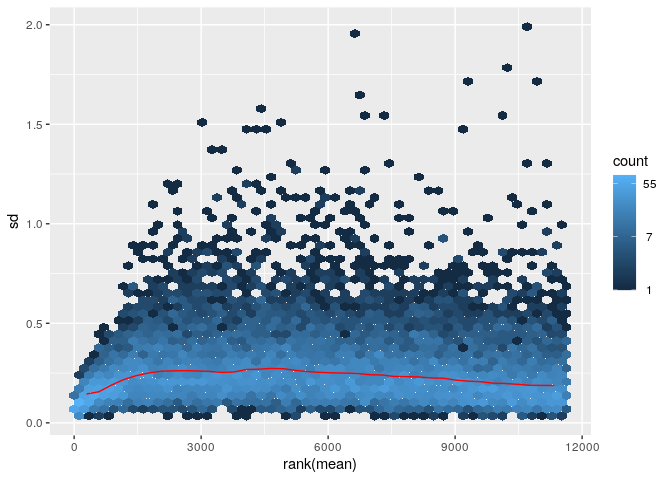
\includegraphics{01_normalisation_files/figure-latex/unnamed-chunk-7-1.pdf}

\begin{Shaded}
\begin{Highlighting}[]
\CommentTok{#if good, normalise data with the trained parameters of vsn}
\NormalTok{count_df_vsn <-}\StringTok{ }\KeywordTok{as.data.frame}\NormalTok{(vsn}\OperatorTok{::}\KeywordTok{predict}\NormalTok{(fit,}\KeywordTok{as.matrix}\NormalTok{(count_df)))}
\end{Highlighting}
\end{Shaded}

We want to avoid finding big fragmentated clusters of points in the
means/sd plot. Here it looks pretty good so we can move forward.

\begin{Shaded}
\begin{Highlighting}[]
\CommentTok{#now let's visualise the normalised data}
\NormalTok{plots <-}\StringTok{ }\KeywordTok{magicPlotMakerLight}\NormalTok{(}\DataTypeTok{df =}\NormalTok{ count_df_vsn, }\DataTypeTok{targets =}\NormalTok{ targets) }
\end{Highlighting}
\end{Shaded}

\begin{verbatim}
## Using ID as id variables
\end{verbatim}

\begin{verbatim}
## Warning: Using alpha for a discrete variable is not advised.
\end{verbatim}

\begin{verbatim}
## Warning: Removed 1 rows containing missing values (geom_text).
\end{verbatim}

\begin{verbatim}
## Warning: Using alpha for a discrete variable is not advised.

## Warning: Using alpha for a discrete variable is not advised.

## Warning: Using alpha for a discrete variable is not advised.
\end{verbatim}

\begin{Shaded}
\begin{Highlighting}[]
\KeywordTok{plot}\NormalTok{(plots[[}\DecValTok{1}\NormalTok{]]) }\CommentTok{#violins}
\end{Highlighting}
\end{Shaded}

\begin{verbatim}
## Warning: Removed 712 rows containing non-finite values (stat_ydensity).
\end{verbatim}

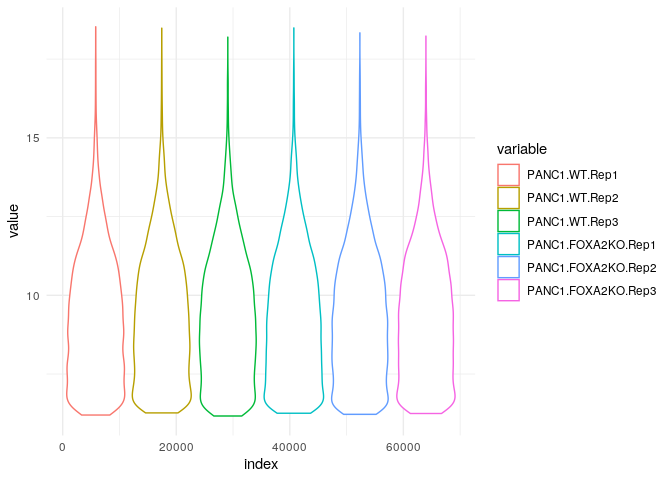
\includegraphics{01_normalisation_files/figure-latex/unnamed-chunk-8-1.pdf}

\begin{Shaded}
\begin{Highlighting}[]
\KeywordTok{plot}\NormalTok{(plots[[}\DecValTok{2}\NormalTok{]]) }\CommentTok{#PCA}
\end{Highlighting}
\end{Shaded}

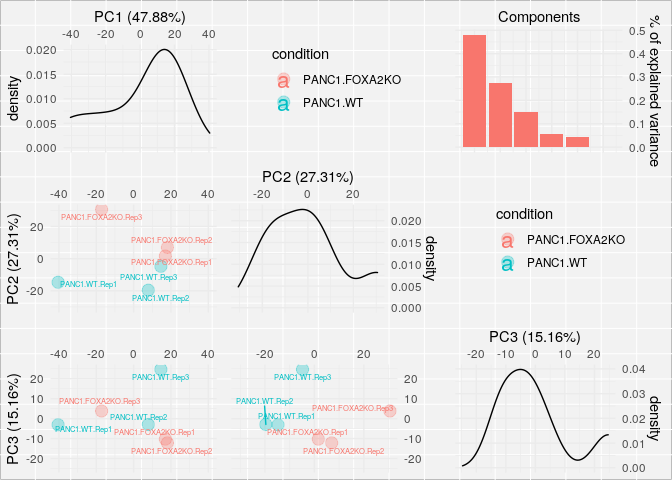
\includegraphics{01_normalisation_files/figure-latex/unnamed-chunk-8-2.pdf}

from PCA, we see that conditions are well seprated by 2nd component. So
it's ok, we will have some signal.

\hypertarget{identifier-kung-fu-optional}{%
\subsubsection{Identifier kung-fu
(optional)}\label{identifier-kung-fu-optional}}

since here with have ensembl id but most our ressources are based on
either uniprot or gene symbole

we need to do some identifer kung-fu

\begin{Shaded}
\begin{Highlighting}[]
\CommentTok{#since here with have ensembl id but most our ressources are based on either uniprot or gene symbole}
\CommentTok{#we need to do some identifer kung-fu}

\CommentTok{#I got this identifer matching dataframe from uniprot}
\NormalTok{gene_id_mapping_from_uniprot <-}\StringTok{ }\KeywordTok{as.data.frame}\NormalTok{(}
  \KeywordTok{read_delim}\NormalTok{(}\StringTok{"support/gene_id_mapping_from_uniprot.tab"}\NormalTok{, }
                                           \StringTok{"}\CharTok{\textbackslash{}t}\StringTok{"}\NormalTok{, }\DataTypeTok{escape_double =} \OtherTok{FALSE}\NormalTok{, }\DataTypeTok{trim_ws =} \OtherTok{TRUE}\NormalTok{))}
\end{Highlighting}
\end{Shaded}

\begin{verbatim}
## Parsed with column specification:
## cols(
##   `yourlist:M201912038471C63D39733769F8E060B506551E125F0C55R` = col_character(),
##   `isomap:M201912038471C63D39733769F8E060B506551E125F0C55R` = col_character(),
##   Entry = col_character(),
##   `Entry name` = col_character(),
##   Status = col_character(),
##   `Protein names` = col_character(),
##   `Gene names` = col_character(),
##   Organism = col_character(),
##   Length = col_double()
## )
\end{verbatim}

\begin{Shaded}
\begin{Highlighting}[]
\NormalTok{gene_id_mapping_from_uniprot <-}\StringTok{ }\NormalTok{gene_id_mapping_from_uniprot[}\OperatorTok{!}\KeywordTok{is.na}\NormalTok{(gene_id_mapping_from_uniprot}\OperatorTok{$}\StringTok{`}\DataTypeTok{Gene names}\StringTok{`}\NormalTok{),]}

\CommentTok{#let's make a pseudo dictionary to make the mapping efficient}
\NormalTok{ensembl_to_symbol <-}\StringTok{ }\KeywordTok{gsub}\NormalTok{(}\StringTok{" .*"}\NormalTok{,}\StringTok{""}\NormalTok{,gene_id_mapping_from_uniprot}\OperatorTok{$}\StringTok{`}\DataTypeTok{Gene names}\StringTok{`}\NormalTok{)}
\KeywordTok{names}\NormalTok{(ensembl_to_symbol) <-}\StringTok{ }\NormalTok{gene_id_mapping_from_uniprot[,}\DecValTok{1}\NormalTok{]}

\CommentTok{#remove all genes that have no gene symbol from our count dataframe}
\KeywordTok{row.names}\NormalTok{(count_df_vsn) <-}\StringTok{ }\KeywordTok{gsub}\NormalTok{(}\StringTok{"[.][0-9]*"}\NormalTok{,}\StringTok{""}\NormalTok{,}\KeywordTok{row.names}\NormalTok{(count_df_vsn))}
\NormalTok{count_df_vsn <-}\StringTok{ }\NormalTok{count_df_vsn[}\KeywordTok{row.names}\NormalTok{(count_df_vsn) }\OperatorTok\StringTok{ }\KeywordTok{names}\NormalTok{(ensembl_to_symbol),]}

\CommentTok{#now let's convert ids with the pseudo dictionary}
\ControlFlowTok{for}\NormalTok{(i }\ControlFlowTok{in} \DecValTok{1}\OperatorTok{:}\KeywordTok{length}\NormalTok{(count_df_vsn[,}\DecValTok{1}\NormalTok{]))}
\NormalTok{\{}
  \KeywordTok{row.names}\NormalTok{(count_df_vsn)[i] <-}\StringTok{ }\NormalTok{ensembl_to_symbol[}\KeywordTok{row.names}\NormalTok{(count_df_vsn)[i]]}
\NormalTok{\}}
\end{Highlighting}
\end{Shaded}

\hypertarget{session-info-details}{%
\subsection{Session Info Details}\label{session-info-details}}

\begin{verbatim}
## R version 3.5.2 (2018-12-20)
## Platform: x86_64-apple-darwin15.6.0 (64-bit)
## Running under: macOS Mojave 10.14.6
## 
## Matrix products: default
## BLAS: /Library/Frameworks/R.framework/Versions/3.5/Resources/lib/libRblas.0.dylib
## LAPACK: /Library/Frameworks/R.framework/Versions/3.5/Resources/lib/libRlapack.dylib
## 
## locale:
## [1] en_US.UTF-8/en_US.UTF-8/en_US.UTF-8/C/en_US.UTF-8/en_US.UTF-8
## 
## attached base packages:
## [1] grid      parallel  stats     graphics  grDevices utils     datasets 
## [8] methods   base     
## 
## other attached packages:
##  [1] hexbin_1.27.3       ggrepel_0.8.1       cowplot_1.0.0      
##  [4] gridExtra_2.3       pheatmap_1.0.12     reshape_0.8.8      
##  [7] ggplot2_3.3.0       vsn_3.50.0          Biobase_2.42.0     
## [10] BiocGenerics_0.28.0 readr_1.3.1        
## 
## loaded via a namespace (and not attached):
##  [1] tidyselect_1.0.0      xfun_0.8              purrr_0.3.3          
##  [4] lattice_0.20-38       colorspace_1.4-1      vctrs_0.2.4          
##  [7] htmltools_0.3.6       yaml_2.2.0            rlang_0.4.5          
## [10] pillar_1.4.3          glue_1.4.0            withr_2.1.2          
## [13] affy_1.60.0           RColorBrewer_1.1-2    affyio_1.52.0        
## [16] lifecycle_0.2.0       plyr_1.8.4            stringr_1.4.0        
## [19] zlibbioc_1.28.0       munsell_0.5.0         gtable_0.3.0         
## [22] evaluate_0.14         labeling_0.3          knitr_1.23           
## [25] fansi_0.4.1           preprocessCore_1.44.0 Rcpp_1.0.4           
## [28] scales_1.1.0          BiocManager_1.30.4    limma_3.38.3         
## [31] farver_2.0.3          hms_0.5.3             digest_0.6.25        
## [34] stringi_1.4.6         dplyr_0.8.5           cli_2.0.2            
## [37] tools_3.5.2           magrittr_1.5          tibble_3.0.0         
## [40] crayon_1.3.4          pkgconfig_2.0.3       ellipsis_0.3.0       
## [43] assertthat_0.2.1      rmarkdown_1.14        R6_2.4.1             
## [46] compiler_3.5.2
\end{verbatim}


\end{document}
